\chapter{NELA-GT-2018 Processing}
\label{app:nela_processing}

We describe here in this appendix our processing to build an additional second dataset for the political leaning classifier used in Chapter~\ref{chap:political_sides}, with random and media splits as the \texttt{Baly} dataset.
The source of the data is the full NELA-GT-2018 dataset, provided in~\citet{DVN/ULHLCB_2019}, which contains $713,534$ news articles coming from $194$ news sources.
Our contribution here is to index it in order to have different splits that can be used then to compare results of political leaning classification.

How a dataset is splitted can greatly affect the results, as we see in~\cite{baly2020we}. Models can learn unwanted patterns and effectively discover shortcuts if the data is not properly segmented.
We provide here both balanced and unbalanced versions of a subset derived from NELA-GT-2018 in two flavours:

\begin{itemize}
    \item random splits: articles from the same news source may appear in all the folds, possibly leading into information leaking;
    \item media splits: articles from a certain news source can only appear in one fold. 
\end{itemize}

\section{Sources Selection}

In order to reduce the dataset, we selected the news sources that have both ratings from AllSides and MBFC telling the same result (excluding the few sources that do not have both, and the ones that have some disagreement).
This results in 65 sources (out of 194) and a total of $286,235$ articles (out of $713,534$).
In this way, we can select the labels from AllSides and we do not need to rely on any mapping strategies between the different labelling systems.

\begin{figure}[!htbp]
    \centering
    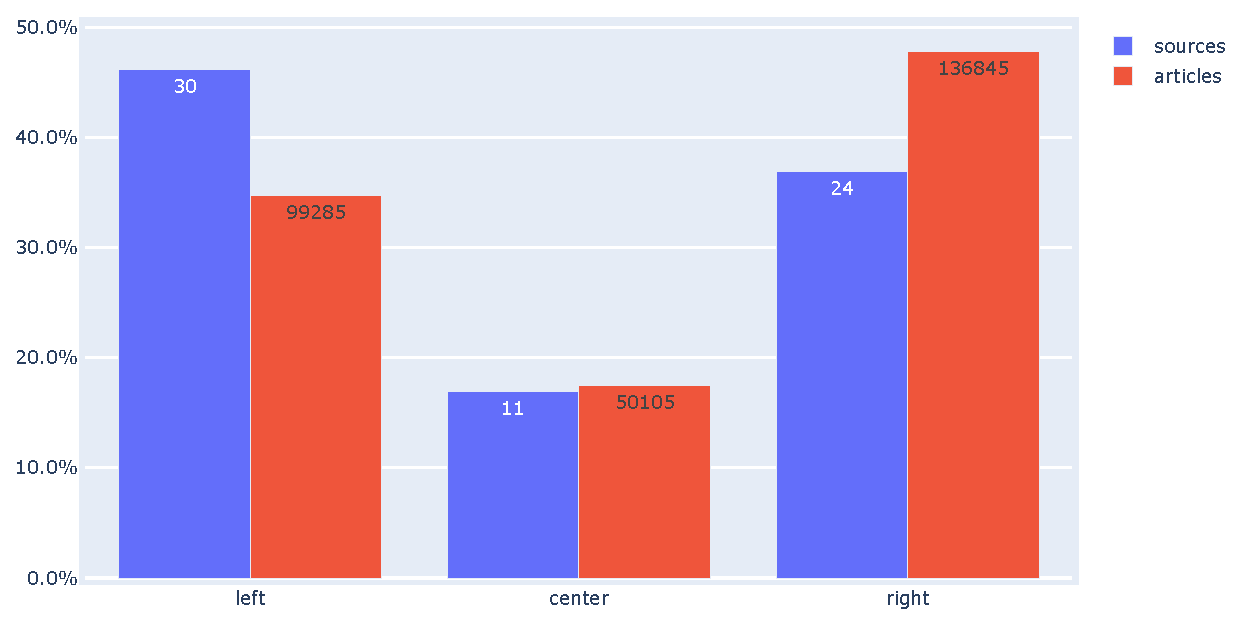
\includegraphics[width=\linewidth]{figures/nela_subset_allsides_simplified.pdf}
    \caption{NELA subset across political leaning}
    \label{fig:nela_subset_allsides_simplified}
\end{figure}

Figure~\ref{fig:nela_subset_allsides_simplified} shows the resulting dataset distribution over political leaning. As we see, this results in a subset that is quite imbalanced. For this reason, we will build subsets that are balanced across political leaning.

With respect to the \texttt{Baly} dataset, we have no relationship between the topics of each leaning, as this dataset comes from unlinked articles (not triples as in \texttt{Baly}). Therefore, even if we balance the splits, we will not have the topics balanced.
Therefore, by testing with this subset, we will see if this becomes a problem or not.

\section{Random Splits Imbalanced}

For the random splits it is less difficult as we have less constraints.
We take the subset identified, and we perform a 5-Folds split, stratified on the leaning.
This strategy is common in the literature as a middle point for reducing the variance of the performance estimate and allowing to use more data for training, and at the same time to avoid too many iterations that require time and resources~\citep{fushiki2011estimation}.

By using a stratified split, we keep the proportion between the number of articles of each leaning. We obtain therefore the \texttt{NELA-Random-Imbalanced} subset.
% We decide to perform a 5-Folds split instead of a simpler 80-20\% train-test split, because we want to avoid the problem of which part of the dataset is selected for testing (which leads to less-generalised results).
% \todoHA{unclear, rewrite}
Instead, by doing a k-folds split, every item of the dataset is used in the test split at different times.
The stratification on the leaning makes every fold with the same proportions across leaning, that is imbalanced but constant.

\section{Random Splits Balanced}

From the \texttt{NELA-Random-Imbalanced} we then derive a balanced version with respect to the leaning. We first identify the leaning that has less articles (center) for each fold, and we cap the number of articles in the other two leanings.
We cannot simply select randomly the articles to remain, because we may lose some of the news sources completely (because the dataset is very unbalanced across news sources).
Therefore, we compute a reduction factor for the Left and one for the Right for each fold (e.g. for $L$=Left and fold=1, $\alpha_{L,1} = \frac{\#articles_{L,1}}{\#articles_{C,1}}$) and we scale proportionally with them the number of articles allowed for each news source in the Left and in the Right. When all these source-based caps have been computed, we then perform a random selection for the articles of each news source.  
We call this subset \texttt{NELA-Random-Balanced}, and it contains $150,315$ articles ($10021$ articles for each fold and leaning).

\section{Media Splits Imbalanced}

Instead for the media splits, we need to keep the constraint that all the news articles from a specific source need to belong to the same fold. In this way, there is no ``leaking" between training and testing, as the models could learn to recognise the style of the source~\citep{baly2020we} and find a shortcut~\citep{geirhos2020shortcut} to the classification problem.

Therefore, the news sources need to be inserted each one in a different fold. At the same time, since there is a big difference between the maximum and minimum number of articles that come from each source, we need to optimize the selection in order to keep the dataset as balanced as possible (even if then we create a balanced version).

% \todoHAinline{This section is not very smooth. It describes datasets but also processing, errors, results, etc. Not easy to follow what your methodology and goals are.}

The greedy strategy that we choose is an adaptation of the Longest-processing-time-first (LPT) algorithm~\citep{graham1969bounds}, that is usually applied in the \emph{minimizing the maximum completion time} problem.
%\todoAW{I'm not really sure what this is about. What are you trying to do?}
The analogy is that the folds are the processors (fixed in number), the goal is to reduce the size of the largest fold instead of reducing the total processing time (with the addition that we have three classes of items that represent the leaning), and the number of articles for each news source corresponds to the processing time of each task.
The only modification is that our objective depends on the total size of each fold, but also on the desired balance also across political leaning.

By applying the LPT greedy algorithm, we first sort the sources by decreasing number of articles. Then, at each iteration, we allocate each source (in the order just computed) to one of the folds. The original LPT allocates to the processor that has the smallest total load. In our case, we allocate to the fold that has the smallest quantity of articles for the leaning of the currently considered source.
This modification to LPT is the consequence of the modified objective stated before.
We prioritize the intra-fold balance across leaning to the inter-fold balance.

% Imbalanced
% articles: [19887, 16416, 33763]	sources: [6, 1, 1]
% articles: [19669, 8360, 25786]	sources: [6, 2, 2]
% articles: [19737, 8492, 25764]	sources: [6, 3, 6]
% articles: [19792, 8386, 25805]	sources: [6, 3, 7]
% articles: [20200, 8451, 25727]	sources: [6, 2, 8]


\begin{table}[!htbp]
    \centering
    \begin{tabular}{l|rrr|rrr}
        \multirow{2}{*}{Fold} & \multicolumn{3}{c}{\#Articles} & \multicolumn{3}{c}{\#Sources} \\
         & Left & Center & Right & Left & Center & Right \\
        \hline
        Fold 1 & 19887 & 16416 & 33763 & 6 & 1 & 1 \\
        Fold 2 & 19669 & 8360 & 25786 & 6 & 2 & 2 \\
        Fold 3 & 19737 & 8492 & 25764 & 6 & 3 & 6 \\
        Fold 4 & 19792 & 8386 & 25805 & 6 & 3 & 7 \\
        Fold 5 & 20200 & 8451 & 25727 & 6 & 2 & 8 \\
    \end{tabular}
    \caption{\texttt{NELA-Media-Imbalanced} across leanings and folds}
    \label{tab:nela_media_imbalanced}
\end{table}

The result of the modified LPT algorithm is shown in Table~\ref{tab:nela_media_imbalanced}, and we name this split with \texttt{NELA-Media-Imbalanced}.
As we can see, the largest source is from the Right with 33763 news articles (\emph{The Sun}, positioned in Fold 1). This causes the most imbalance in our situation. However, the greedy algorithm places it as the first one, and then manages to pull together 6 sources from the Left that sum up to 19887 news articles.
We see that overall the folds are quite balanced, with this exception of the Right in Fold 1, and the Center between Fold 1 and the other folds.

\section{Media Splits Balanced}

The last splitting subset that we create is derived from \texttt{NELA-Media-Imbalanced}, but adding the constraint of being balanced across leaning.
For each fold, we take the minimum number of articles (always the Center) and, as in \texttt{NELA-Media-Balanced}, we compute a reduction factor for the Left and one for the Right for each fold. Then we scale proportionally with these factors the number of articles allowed for each news source in the Left and in the Right. When all these source-based caps have been computed, we then perform a random selection for the articles of each news source.  

\begin{table}[!htbp]
    \centering
    \begin{tabular}{l|rrr|rrr}
        \multirow{2}{*}{Fold} & \multicolumn{3}{c}{\#Articles} & \multicolumn{3}{c}{\#Sources} \\
         & Left & Center & Right & Left & Center & Right \\
        \hline
        Fold 1 & 16416 & 16416 & 16416 & 6 & 1 & 1 \\
        Fold 2 & 8360 & 8360 & 8360 & 6 & 2 & 2 \\
        Fold 3 & 8492 & 8492 & 8492 & 6 & 3 & 6 \\
        Fold 4 & 8386 & 8386 & 8386 & 6 & 3 & 7 \\
        Fold 5 & 8451 & 8451 & 8451 & 6 & 2 & 8 \\
    \end{tabular}
    \caption{\texttt{NELA-Media-Balanced} across leanings and folds}
    \label{tab:nela_media_balanced}
\end{table}

Table~\ref{tab:nela_media_balanced} shows the result of the balancing, where the first fold results being the largest one as its limit (number of articles in the Center) is higher.
We call this subset \texttt{NELA-Media-Balanced}.

% We will use all these subsets in the following Section~\ref{ssec:ps_prop_leaning_classifier} in order to see if the results generalise or not to other datasets.
The splits produced with this methodology are used in Chapter~\ref{ssec:ps_prop_leaning_classifier}.
